% ----------------------------------------------------------
% Introdução (exemplo de capítulo sem numeração, mas presente no Sumário)
% ----------------------------------------------------------
\chapter[Introdução]{Introdução}
%\addcontentsline{toc}{chapter}{Introdução}
% ----------------------------------------------------------
 Dentre os diversos processos de uma usina integrada, podemos destacar que na Aciaria, temos o processo dos convertedores, que de acordo com \cite{machado2003siderurgia}, é o processo no qual ocore a transformação do gusa líquido em aço que envolve:

\begin{itemize}
	\item a diminuição dos teores de carbono, silício, fósforo, enxofre e nitrogênio a níveis bastante baixos;
	\item a adição de sucata ou minério de ferro para ajustar a temperatura do aço bruto;
	\item o ajuste dos teores de carbono, manganês, elementos de liga e da temperatura no forno ou na panela de vazamento;
\end{itemize}

Posteriormente, destaca-se a etapa de lingotamento contínuo na qual o aço é convertido do estado líquido para o sólido através da Máquina de Lingotamento Contínuo (MLC), dando origem a produtos semi-acabados, como perfis, placas, blocos ou tarugos.

\begin{figure}[htbp]
	\centering
	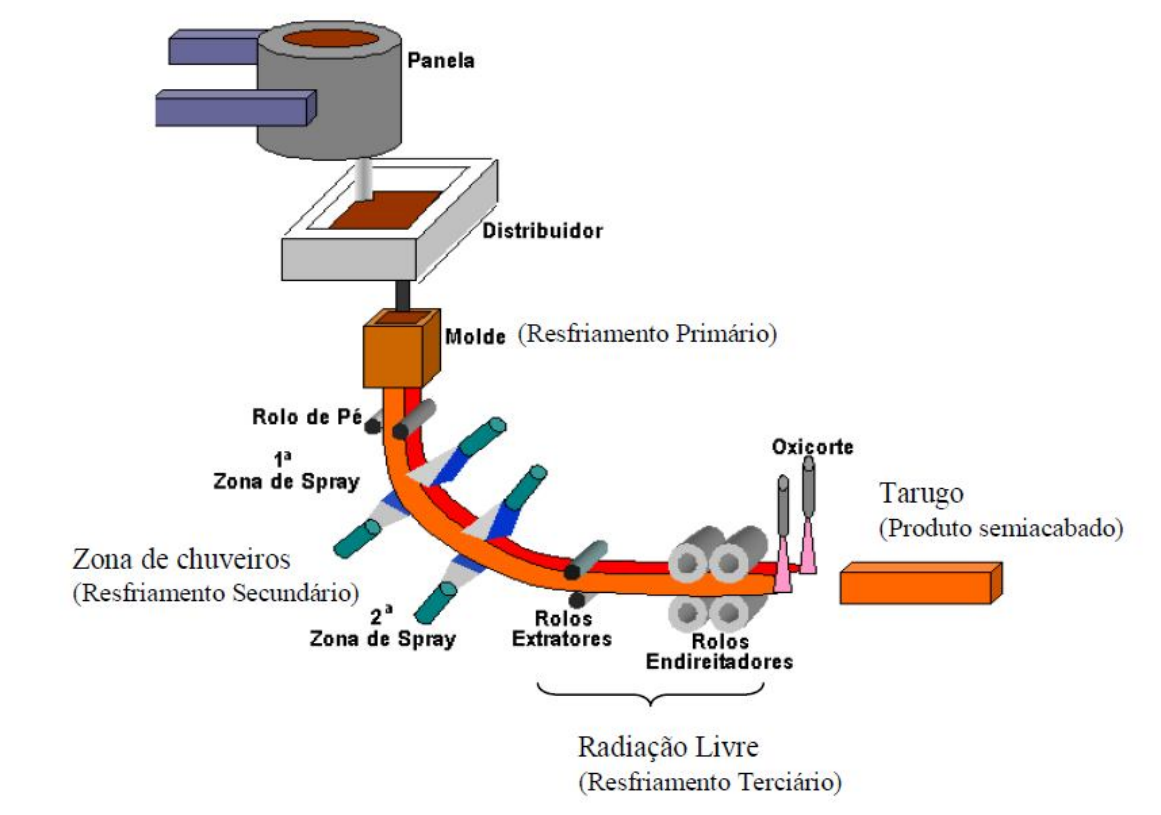
\includegraphics[width=0.8\linewidth]{figuras/Steel/artigo_2.png}
	\caption{Processo de lingotamento Contínuo de Tarugos}
	\legend{Fonte: \citeauthor{freitas2013analise} (\citeyear{freitas2013analise})}
	\label{fig:processLing}
\end{figure}

Como mostrado na Figura \ref{fig:processLing}, o processo de Lingotamento Contínuo de Tarugo se inicia quando uma panela que contém, em média, 224 toneladas de aço chega à plataforma com temperaturas ideias, em torno de 1500 ºC, para ser lingotada de forma que o equipamento possa efetuar horas ou ate mesmo dias de produção sem interrupção. Cada panela que é lingotada, da-se o nome de \textbf{corrida}. 

A etapa de solificação ocorre de fora para dentro do veio em função do contato com as paredes refrigeradas do molde, aspersão de água em sprays e perda de calor por radiação para o ambiente. Essa troca de calor faz com que o aço se solidifique gradativamente criando zonas onde o material pode ser encontrado em seus estados sólido e líquido.

No processo final de cada corrida, os tarugos são cortados na máquina Oxicorte como mostrado na Figura \ref{fig:processLing}. Os cortes são feitos de acordo com a demanda do cliente e origina em média 100 tarugos, número este que depende do diâmetro das peças que podem ser todas de 130mm ou 160mm e do comprimento das mesmas que variam de 07 a 14m. Após serem cortados são transportados para o despacho, por uma ponte rolante a base de eletroímãs que suportam altas temperaturas e 27 toneladas de carga. 


\begin{figure}[htbp]
	\centering
	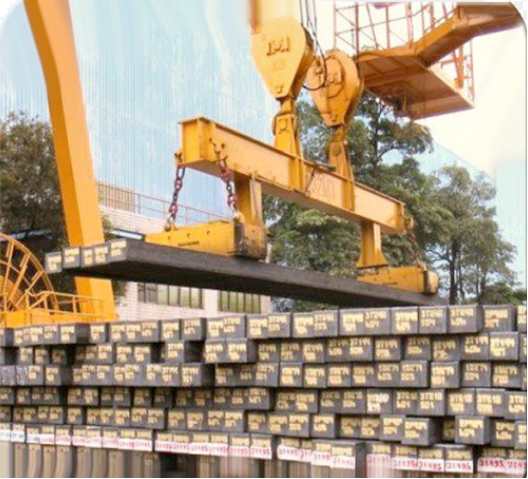
\includegraphics[width=0.7\linewidth]{figuras/Steel/ponte_rolante.png}
	\caption{Ponte Rolante}
	\legend{Fonte: \citeauthor{ponte-rolante} (\citeyear{ponte-rolante})}
	\label{fig:crane}
\end{figure}

\begin{figure}[htbp]
	\centering
	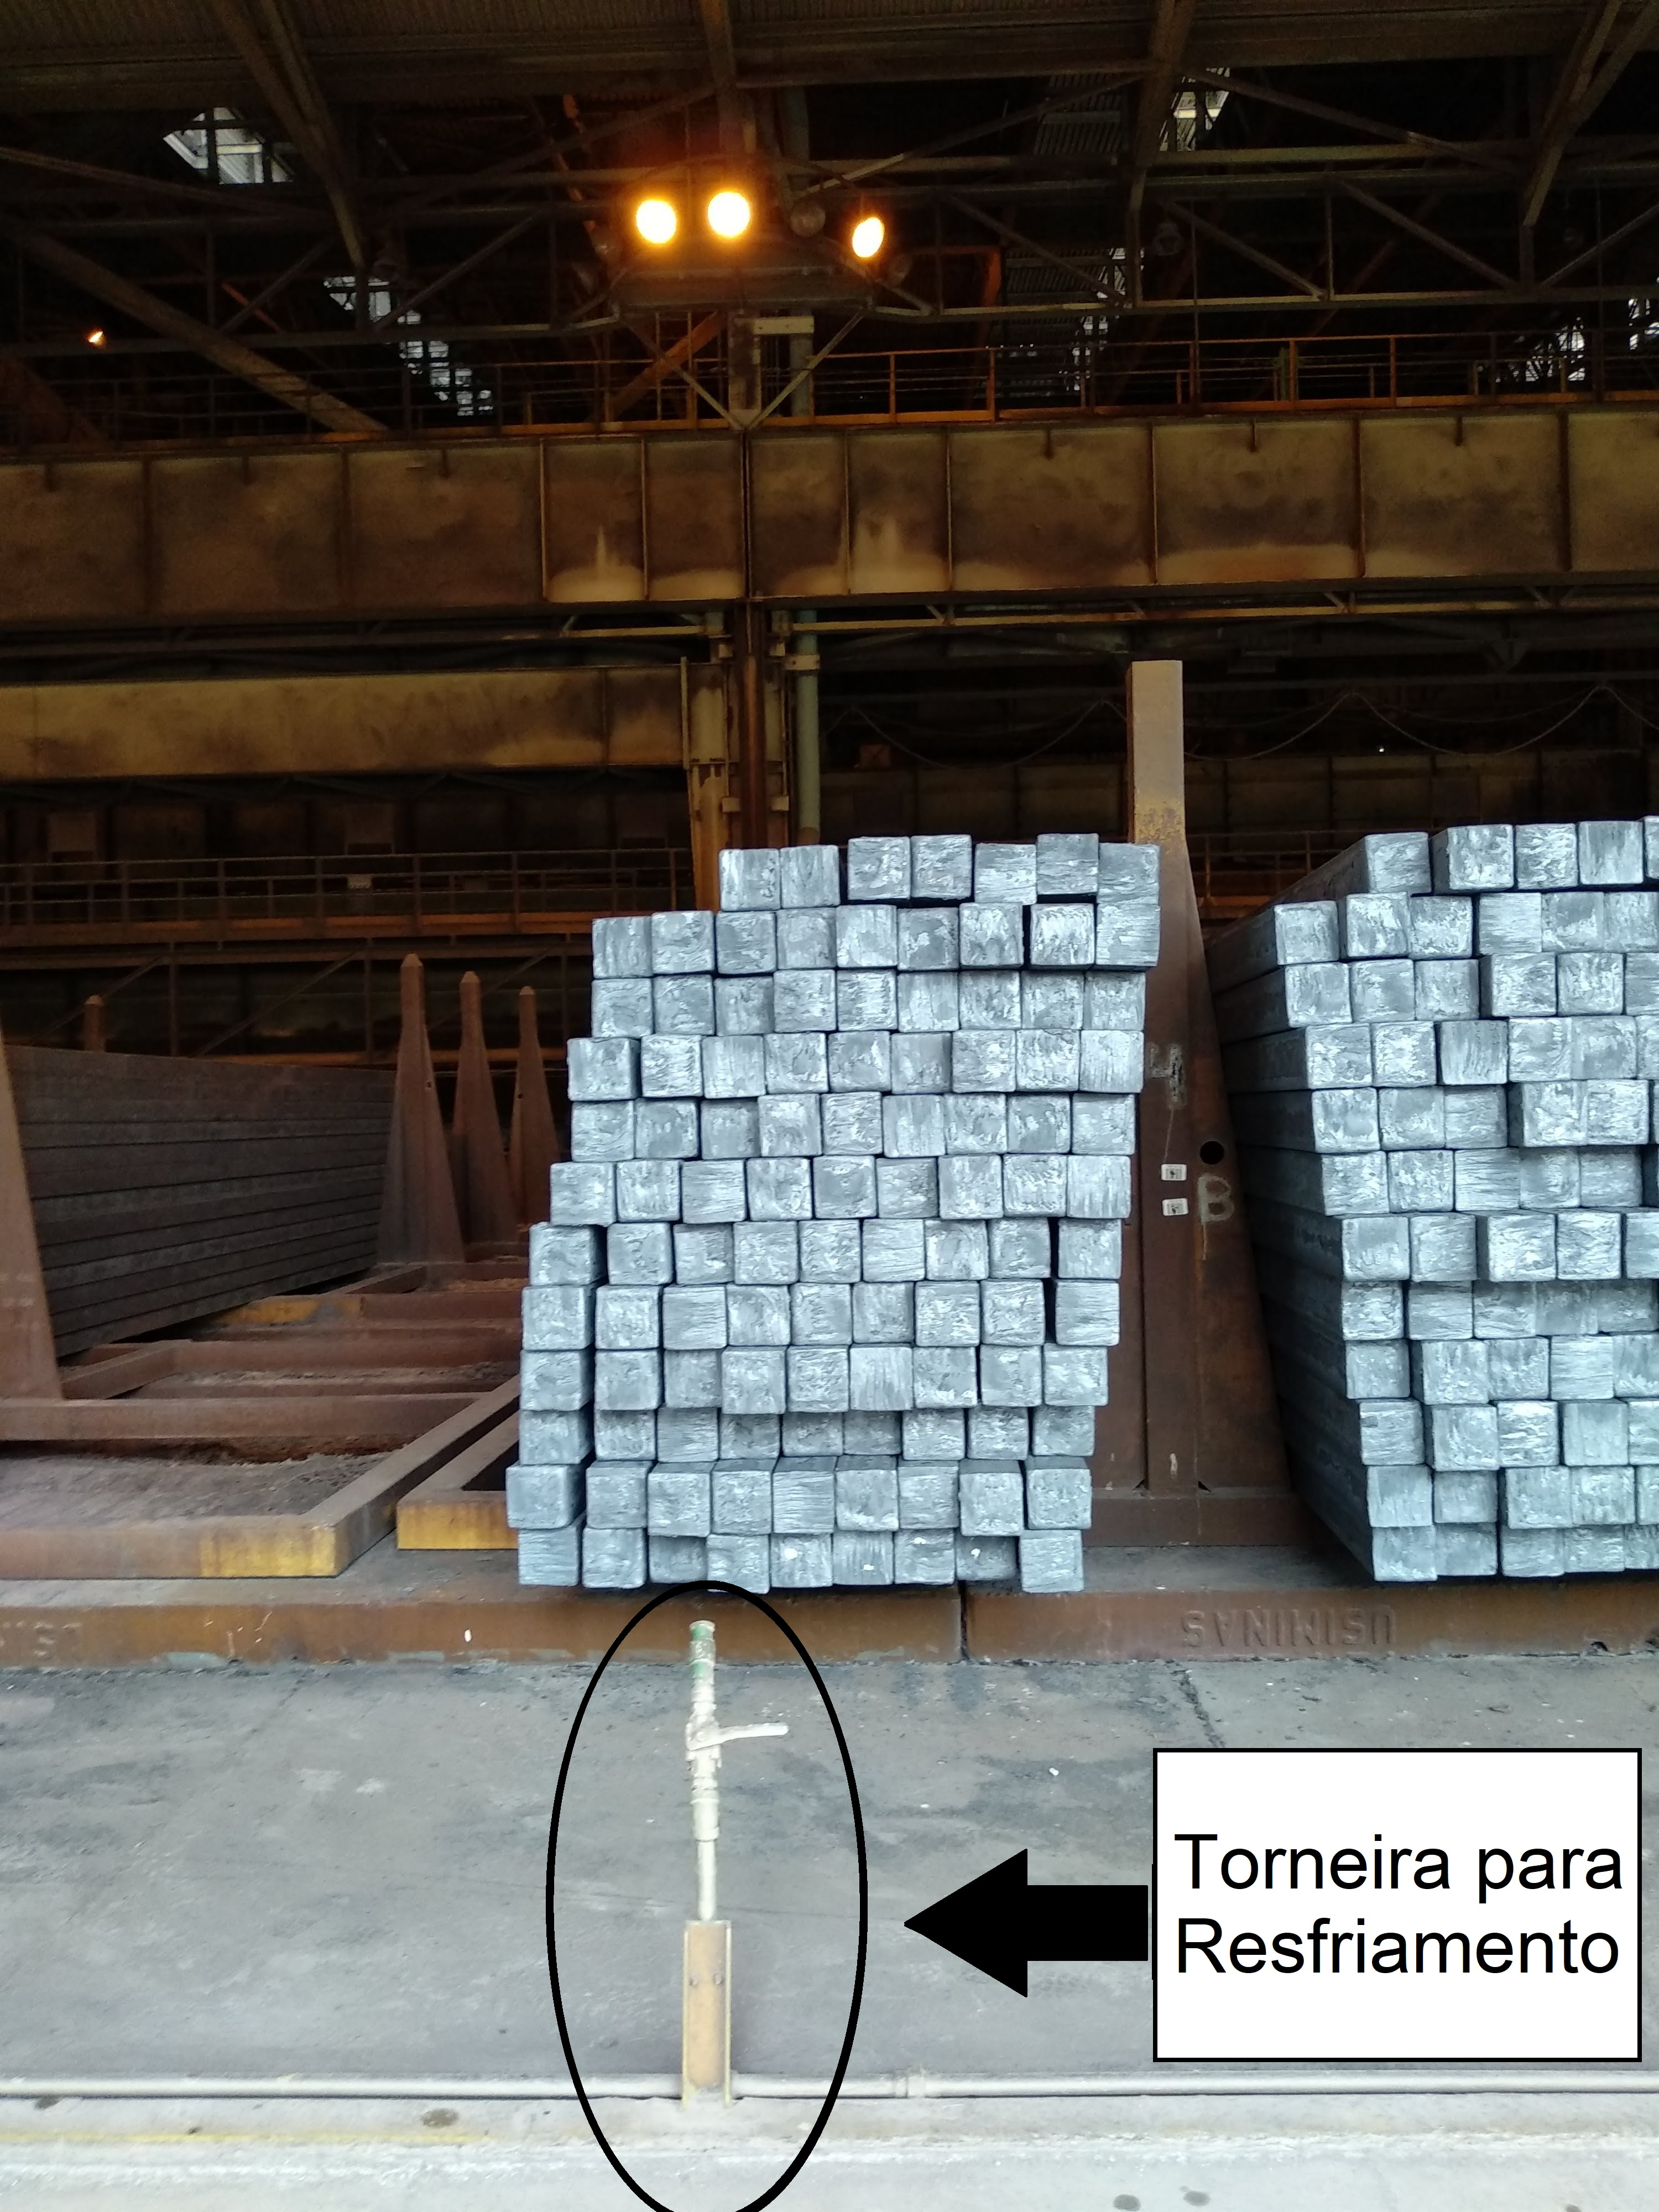
\includegraphics[width=0.5\linewidth]{figuras/Steel/despacho.jpg}
	\caption{Despacho}
	\label{fig:despacho}
\end{figure}

Uma vez que os tarugos são colocados no despacho, no qual se encontram em uma temperatura média de 700 ºC, eles precisam esperar em torno de 15 a 20 horas até que fiquem em uma temperatura ideal (média de 150 ºC) e o operador possa pregar a etiqueta metálica de identificação. Para ajudar no resfriamento dos tarugos, é colocado sobre eles um jato de água através de uma torneira como mostrado na Figura \ref{fig:despacho} com uma frequencia constante apenas na face frontal, pois se a água for colocada diretamente no centro do tarugo irá empená-lo, uma vez que a temperatura central do tarugo ainda está muito mais quente que as extremidades.

Após esperar o tempo necessário para que o tarugo chegue na temperatura ideial, o operador responsável faz a impressão das etiquetas metálicas. Para que as etiquetas sejam pregadas com segurança, é utilizado Silicone Acético Transparente, no qual foi testada e comprovada sua eficácia na restência sobre alta temperatura. 

\begin{figure}[htbp]
	\centering
	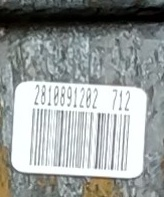
\includegraphics[width=0.25\linewidth]{figuras/Steel/barcode.jpg}
	\caption{Etiqueta}
	\label{fig:barcode}
\end{figure}

A rotulação dos tarugos é muito importante para que possa ser feita a rastreabilidade e a identificação do aço em processos posteriores como, por exemplo, na laminação até o cliente final. 
%A composição dos números intrinsecos ao códico de barra impresso na etiqueta metálica, como da Figura \ref{fig:barcode}, é o que permite a identificação supracitada a saber:

\begin{table}[]
	\centering
	\begin{tabular}{|l|l|}
		\hline
		\rowcolor[HTML]{ECF4FF} 
		\multicolumn{1}{|c|}{\cellcolor[HTML]{ECF4FF}Número} & \multicolumn{1}{c|}{\cellcolor[HTML]{ECF4FF}2810891202 712}\\ \hline
		28 & Número do convertedor que pode ser CV1 (27) ou CV2 (28).\\ \hline
		10891202 & Número da corrida no qual: \cr & 10: Quantidade de carbono 
		                                      \cr &  \\ \hline
        712 & Número 7 é o veio que a peça foi lingotada e 12 o número da peça.\\ \hline
	\end{tabular}
	\caption{Significado dos dígitos da etiqueta de rotulação.}
	\label{tab:tag}
\end{table}

Vale ressaltar que o número de identificação da etiqueta pode ser reconhecido pelos dígitos ou pelo código de barras através de um leitor. Em cada etiqueta o código de barras e os dígitos acima deste correspondem à mesma sequência numérica.

Hoje em dias os problemas referente ao procedimento de identificação de peças se dão pelo fato de que:
\begin{enumerate}
	\item O operador responsável pela rotuação precisa contar o número de tarugos existentes na pilha e conferir cada etiqueta se está certa com sistema, anotar e informar a quantia para sala de operação para que o operador da sala de controle valide com sistema de contagem de peças da MLC. Isso pode acarretar em erros humanos.
	\item O local em que a pilha de peças se encontra é perigoso devido ao fato de, a todo momento, uma ponte rolante estar trabalhando no mesmo local.
\end{enumerate}

\section{Objetivos} 

O objetivo deste trabalho é desenvolver um sistema, de baixo custo, baseado nas tecnologias de \textit{Machine Learning}, Microserviços, Desenvolvimento Web e \textit{Cloud Computing} para automatizar o processo e reduzir o erro humano através da integração entre uma câmera e camadas de softwares. 

O sistema, através de uma foto, será capaz de identificar as etiquetas fixadas no Tarugo, contar o número de etiquetas, identificar o código de barras que se econtra nelas e, além disso, identificar os números que se encontram acima do mesmo.

Será criado uma aplicação Web com um servidor \textit{online} para que o usuário final possa administrar o sistema através de telas com um \textit{layout} mais amigável.

\subsection{Objetivos específicos}

\begin{itemize}
	\item Recolher várias imagens contendo todos os Tarugos;
	\item Implementar o sistema de expansão dos \textit{datasets} através do método \textit{Data Augmentation}, para que a quantidade de imagens seja suficiente para treinar os modelos de \textit{Machine Learning};
	\item Treinar e implementar o modelo de reconhecimento de código de barras;
	\item Treinar e implementar o modelo de reconhecimento de números;
	\item Implementar a aplicação Web;
	\item Publicar a aplicação no Google Cloud Plataform;
	\item Integrar todos os sistemas a fim de garantir as funcionalidades do projeto;
	\item Executar os procedimentos em ambiente online a fim de validar o projeto;
\end{itemize}

%\section{Justificativas e Relev{\^a}ncia}

\section{Organização do trabalho}

O presente trabalho está organizado em X capítulos. No Capítulo 1, encontra-se ... 